% Compile with latexmk -pdf, or run pdflatex twice: long tables settle their column widths in the second run.
\documentclass[a4paper]{article}

\usepackage[margin=1in]{geometry}
\usepackage[T1]{fontenc}
\usepackage{graphicx}
\usepackage{booktabs}
\usepackage{longtable}
\usepackage{needspace}
\usepackage{array}
\usepackage{amsmath}
\usepackage{tikz}
\usepackage{pgfplots}
\usepackage{paralist}
\usepackage{url}
\pgfplotsset{compat=1.16}
\setlength{\tabcolsep}{4pt}

\begin{document}

\noindent
Factor analysis of the dataset ``Important Factors: Inductive miner'', exported from Complexity Factor Analysis on 2026-10-21T00:00:00+00:00.

\section*{Chosen Discovery Algorithms}
For this factor analysis, the following miners discovered the process models:
\begin{compactitem}
\item Inductive miner
\end{compactitem}

This means, for each input event log, a model was discovered with each of the aforementioned discovery algorithms.
For the resulting Petri nets, the complexity score of each selected measure was calculated, which formed the population.

The following complexity measures were analysed:
\begin{compactitem}
\item Size
\item Connector Mismatch
\item Connector Heterogeneity
\item Token split
\item Control flow complexity
\item Separability
\item Average connector degree
\item Maximum connector degree
\item Sequentiality
\item Coefficient of network connectivity
\item Density
\item Number of duplicate tasks
\item Number of empty sequence flows
\end{compactitem}

\noindent
Before the analysis, the following measures were left out:
\begin{compactitem}
\item Number of empty sequence flows: no variance
\end{compactitem}

\section*{Validity of the Factor Analysis}
The sample size in this analysis was $288$.
It is recommended to have a sample size of at least $5 \cdot 13 = 65$.

Bartlett's test of sphericity returned a $\chi^2$ value of $6822.4414$ ($66$ degrees of freedom) and a $p$-value of $0$.
This means, the variables are probably correlated and we can perform a factor analysis.

\noindent
The measure of sampling adequacy (MSA) returned the following results:
\begin{compactitem}
\item Size: $0.6913$
\item Connector Mismatch: $0.7634$
\item Connector Heterogeneity: $0.7023$
\item Token split: $0.8338$
\item Separability: $0.6196$
\item Average connector degree: $0.7744$
\item Maximum connector degree: $0.6671$
\item Coefficient of network connectivity: $0.7982$
\item Density: $0.7559$
\item Number of duplicate tasks: $0.7438$
\item overall MSA: $0.7467$
\end{compactitem}

\noindent
During the analysis, the MSA values of the following complexity measures were too low (below $0.60$), in the round of the filter that removed them:
\begin{compactitem}
\item Sequentiality: $0.4889$ (round 1)
\item Control flow complexity: $0.5730$ (round 1)
\end{compactitem}

These complexity measures were left out of the analysis to produce dependable results.

\section*{Chosen Number of Factors}
\noindent
The Scree test resulted in the following Eigenvalue plot:
\begin{center}
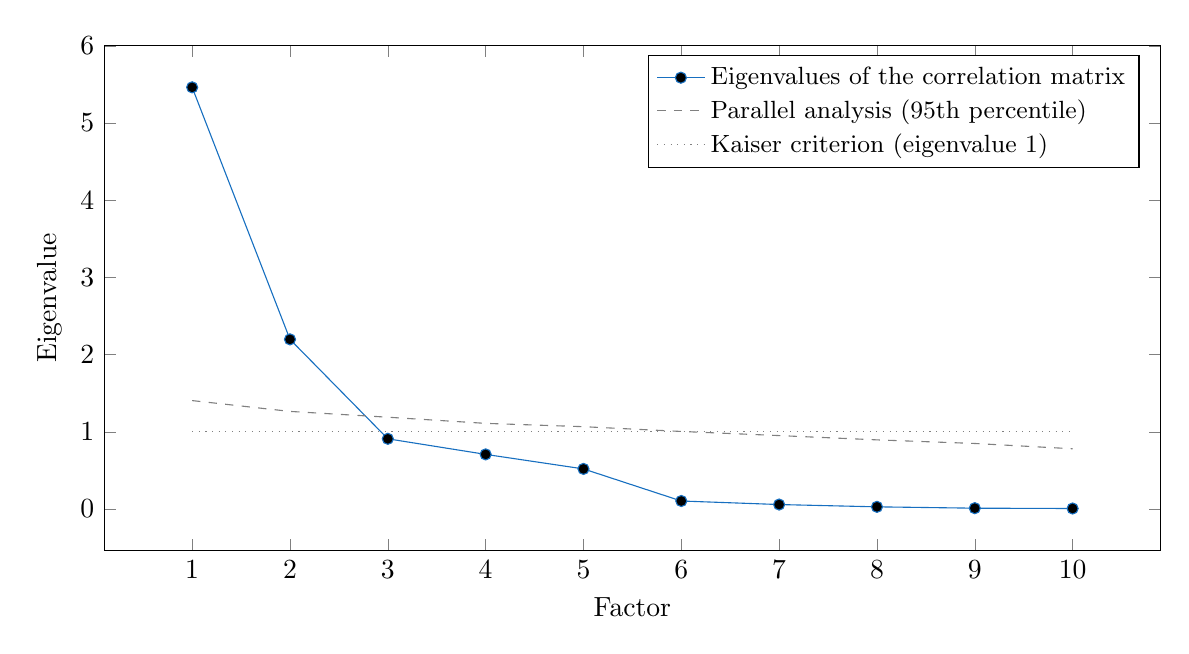
\begin{tikzpicture}
\begin{axis}[xtick=data,width=15cm,height=8cm,xlabel={Factor},ylabel={Eigenvalue},legend cell align=left,legend style={font=\small}]
\addplot [draw=cyan!50!blue, mark=*] coordinates { (1,5.4620) (2,2.1971) (3,0.9091) (4,0.7073) (5,0.5192) (6,0.1034) (7,0.0576) (8,0.0278) (9,0.0103) (10,0.0063) };
\addlegendentry{Eigenvalues of the correlation matrix}
\addplot [draw=gray, dashed, mark=none] coordinates { (1,1.4043) (2,1.2640) (3,1.1889) (4,1.1091) (5,1.0661) (6,1.0043) (7,0.9508) (8,0.8953) (9,0.8486) (10,0.7800) };
\addlegendentry{Parallel analysis (95th percentile)}
\addplot [draw=gray, dotted, mark=none, domain=1:10, samples=2] {1};
\addlegendentry{Kaiser criterion (eigenvalue 1)}
\end{axis}
\end{tikzpicture}
\end{center}

\needspace{12\baselineskip}
\noindent
The share of the variance of each component is its eigenvalue divided by the number of measures, $10$, as ComFy plots it:
\begin{center}
\begin{tabular}{rrrr}
\toprule
Factor & Eigenvalue & Share of variance & Parallel analysis \\
\midrule
1 & $5.4620$ & $0.5462$ & $1.4043$ \\
2 & $2.1971$ & $0.2197$ & $1.2640$ \\
3 & $0.9091$ & $0.0909$ & $1.1889$ \\
4 & $0.7073$ & $0.0707$ & $1.1091$ \\
5 & $0.5192$ & $0.0519$ & $1.0661$ \\
6 & $0.1034$ & $0.0103$ & $1.0043$ \\
7 & $0.0576$ & $0.0058$ & $0.9508$ \\
8 & $0.0278$ & $0.0028$ & $0.8953$ \\
9 & $0.0103$ & $0.0010$ & $0.8486$ \\
10 & $0.0063$ & $0.0006$ & $0.7800$ \\
\bottomrule
\end{tabular}
\end{center}

The number of expected factors was set to $4$; the Kaiser criterion suggests $2$, parallel analysis $2$ (100 samples of random normal data, seed 20261012). The factors were fitted with minres and the varimax rotation.

\section*{Descriptive Statistics}
\noindent
Over all $288$ observations of the data as collected, before any measure was left out; missing values are not counted. Std is the sample standard deviation ($n - 1$ in the denominator).

\begin{center}
\begin{tabular}{lrrrrr}
\toprule
 & Mean & Median & Std & Min & Max \\
\midrule
Size & 71.684028 & 56.000000 & 36.639797 & 34.000000 & 197.000000 \\
Connector Mismatch & 0.295139 & 0.000000 & 0.773951 & 0.000000 & 6.000000 \\
Connector Heterogeneity & 0.468514 & 0.580907 & 0.288524 & 0.000000 & 0.876716 \\
Token split & 4.097222 & 2.000000 & 4.568975 & 0.000000 & 18.000000 \\
Control flow complexity & 42.496528 & 40.000000 & 14.780625 & 9.000000 & 89.000000 \\
Separability & 0.974704 & 0.980000 & 0.026153 & 0.900000 & 1.000000 \\
Average connector degree & 7.332361 & 5.277174 & 5.116867 & 2.857143 & 20.000000 \\
Maximum connector degree & 16.972222 & 18.000000 & 7.826912 & 3.000000 & 34.000000 \\
Sequentiality & 0.975604 & 1.000000 & 0.059853 & 0.706897 & 1.000000 \\
Coefficient of network connectivity & 1.496595 & 1.496667 & 0.195798 & 1.105263 & 1.818182 \\
Density & 0.089553 & 0.057416 & 0.077884 & 0.013514 & 0.250000 \\
Number of duplicate tasks & 20.524306 & 11.000000 & 20.104763 & 0.000000 & 81.000000 \\
Number of empty sequence flows & 0.000000 & 0.000000 & 0.000000 & 0.000000 & 0.000000 \\
\bottomrule
\end{tabular}
\end{center}

\section*{Results of the Factor Analysis}
\begin{center}
\begin{tabular}{lccccc}
\toprule
 & Factor 1 & Factor 2 & Factor 3 & Factor 4 & $h^2$ \\
\midrule
Size & $\mathbf{0.9712}$ & \textcolor{lightgray}{$-0.1515$} & \textcolor{lightgray}{$-0.1211$} & \textcolor{lightgray}{$0.1158$} & $0.9943$ \\
Connector Mismatch & \textcolor{lightgray}{$0.2446$} & \textcolor{lightgray}{$-0.2312$} & \textcolor{lightgray}{$-0.2256$} & \textcolor{lightgray}{$0.2028$} & $0.2053$ \\
Connector Heterogeneity & \textcolor{lightgray}{$-0.0123$} & \textcolor{lightgray}{$-0.1617$} & $\mathbf{-0.9338}$ & \textcolor{lightgray}{$-0.2060$} & $0.9407$ \\
Token split & $\mathbf{0.9516}$ & \textcolor{lightgray}{$-0.2000$} & \textcolor{lightgray}{$-0.0740$} & \textcolor{lightgray}{$0.0142$} & $0.9513$ \\
Separability & \textcolor{lightgray}{$0.2051$} & \textcolor{lightgray}{$0.1520$} & \textcolor{lightgray}{$0.2582$} & $\mathbf{0.6252}$ & $0.5228$ \\
Average connector degree & $\mathbf{-0.4835}$ & $\mathbf{0.4608}$ & $\mathbf{0.5830}$ & $0.4128$ & $0.9564$ \\
Maximum connector degree & \textcolor{lightgray}{$-0.1844$} & $\mathbf{0.9532}$ & \textcolor{lightgray}{$0.1908$} & \textcolor{lightgray}{$0.1303$} & $0.9961$ \\
Coefficient of network connectivity & $-0.4728$ & $\mathbf{0.6628}$ & \textcolor{lightgray}{$0.2911$} & $0.4778$ & $0.9759$ \\
Density & $\mathbf{-0.5808}$ & \textcolor{lightgray}{$0.3288$} & $\mathbf{0.6126}$ & $0.4010$ & $0.9815$ \\
Number of duplicate tasks & $\mathbf{0.9721}$ & \textcolor{lightgray}{$-0.1978$} & \textcolor{lightgray}{$-0.0557$} & \textcolor{lightgray}{$0.0831$} & $0.9941$ \\
\midrule
SS loadings & $3.7246$ & $1.8732$ & $1.8490$ & $1.0715$ & \\
Proportion & $0.3725$ & $0.1873$ & $0.1849$ & $0.1071$ & \\
Cumulative & $0.3725$ & $0.5598$ & $0.7447$ & $0.8518$ & \\
\bottomrule
\end{tabular}
\end{center}

\noindent
Loadings of the 4 factor(s). Bold: the loadings by which the assignment rule puts a measure on a factor. Grey: loadings that do not count, $|\lambda| \leq 0.35$; a loading counts with $|\lambda| > 0.35$. $h^2$ is the communality.

\section*{Communalities}
\begin{center}
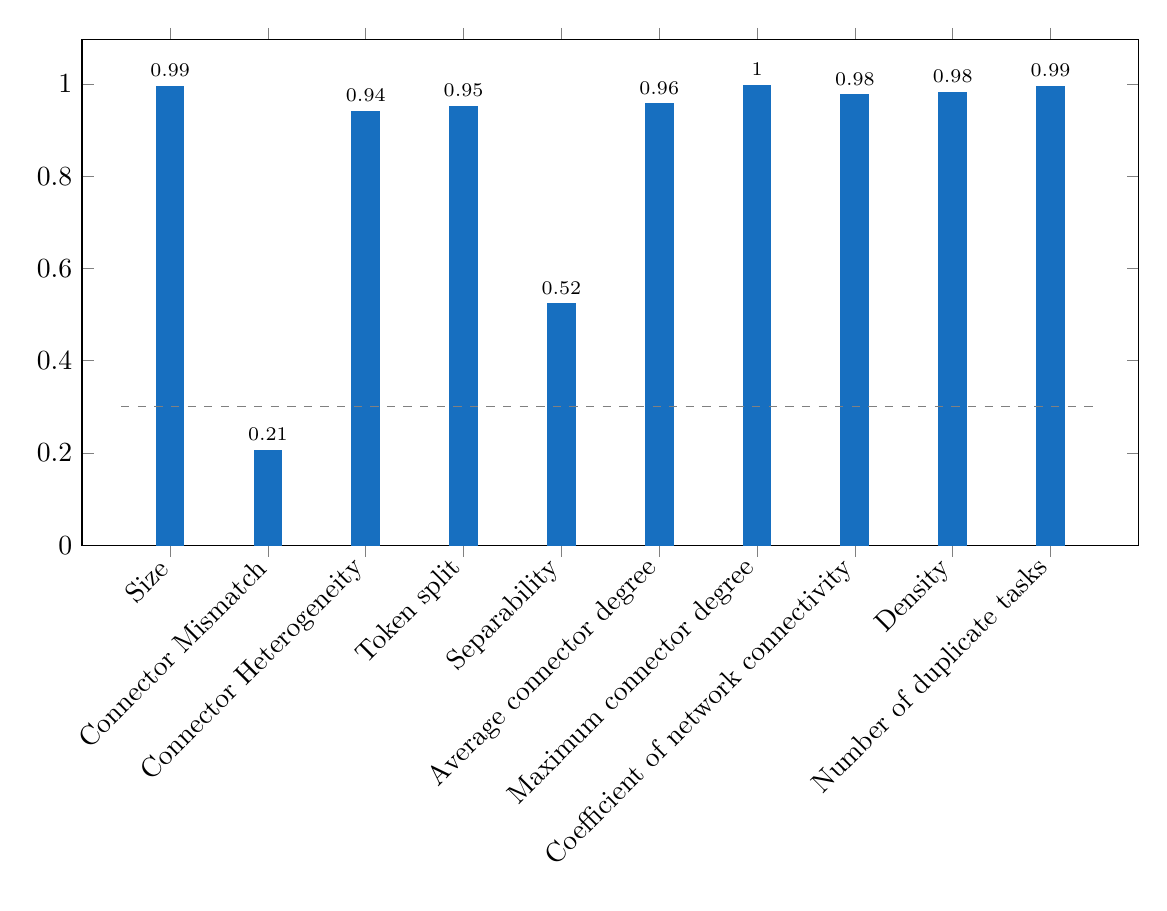
\begin{tikzpicture}
\begin{axis}[ybar,ymin=0,xtick=data,xticklabels={{Size},{Connector Mismatch},{Connector Heterogeneity},{Token split},{Separability},{Average connector degree},{Maximum connector degree},{Coefficient of network connectivity},{Density},{Number of duplicate tasks}},xticklabel style={rotate=45, anchor=east},nodes near coords={\pgfmathprintnumber{\pgfplotspointmeta}},every node near coord/.append style={font=\scriptsize},width=15cm,height=8cm]
\addplot [draw=cyan!50!blue, fill=cyan!50!blue] coordinates { (1,0.9943) (2,0.2053) (3,0.9407) (4,0.9513) (5,0.5228) (6,0.9564) (7,0.9961) (8,0.9759) (9,0.9815) (10,0.9941) };
\draw [gray, dashed] (axis cs:0.5,0.30) -- (axis cs:10.5,0.30);
\end{axis}
\end{tikzpicture}
\end{center}
The dashed line marks the communality an assigned measure needs, $0.30$.

\needspace{12\baselineskip}
\section*{Dimensions}
\noindent
The assignment rule ``multi'' puts each measure on every factor whose absolute loading exceeds the threshold and lies at most 0.15 below its largest (Important Factors, after Lieben et al.).

\begin{longtable}{@{}>{\raggedright\arraybackslash}p{4.5cm}>{\raggedright\arraybackslash}p{11cm}@{}}
\toprule
Factor & Measures (loading) \\
\midrule
\endhead
\bottomrule
\endfoot
Factor 1 & Number of duplicate tasks ($0.97$), Size ($0.97$), Token split ($0.95$), Density ($-0.58$), Average connector degree ($-0.48$) \\
Factor 2 & Maximum connector degree ($0.95$), Coefficient of network connectivity ($0.66$), Average connector degree ($0.46$) \\
Factor 3 & Connector Heterogeneity ($-0.93$), Density ($0.61$), Average connector degree ($0.58$) \\
Factor 4 & Separability ($0.63$) \\
\end{longtable}

\noindent
In no factor:
\begin{compactitem}
\item Connector Mismatch: low communality
\end{compactitem}

\noindent
Cross-loadings, loadings at most $0.15$ below the largest one of a measure:
\begin{compactitem}
\item Average connector degree: Factor 3 ($0.58$), Factor 1 ($-0.48$), Factor 2 ($0.46$)
\item Density: Factor 3 ($0.61$), Factor 1 ($-0.58$)
\end{compactitem}

\needspace{12\baselineskip}
\section*{Settings and Provenance}
\begin{center}
\begin{tabular}{@{}>{\raggedright\arraybackslash}p{4.2cm}>{\raggedright\arraybackslash}p{11.3cm}@{}}
\toprule
Setting & Value \\
\midrule
Dataset & Important Factors: Inductive miner (model measures, source bundled) \\
Observations & $288$ of the cleaned matrix \\
Measures excluded by hand & none \\
MSA filter & on, threshold $0.60$ \\
Significance level & $\alpha = 0.05$ for Bartlett's test \\
Number of factors & $4$ (set by hand) \\
Rotation & varimax \\
Loading threshold & $|\lambda| > 0.35$ \\
Communality threshold & $h^2 \geq 0.30$ \\
Assignment rule & multi: each measure on every factor whose absolute loading exceeds the threshold and lies at most 0.15 below its largest (Important Factors, after Lieben et al.) \\
Method & minres with factor\_analyzer 0.5.1 \\
Parallel analysis & 100 samples of random normal data, 95th percentile, seed 20261012 \\
Measure names & full names \\
Data & bundled dataset comfy-paper-inductive-miner, from https://github.com/Pati-nets/ComFy, commit 1dd6ea6 \\
Software & Complexity Factor Analysis (version v0.0.0, commit 000000000000); factor\_\allowbreak{}analyzer 0.5.1 \\
Source code & \url{https://github.com/Magiertx/complexity-factor-analysis} \\
Citation & Data of the paper ``Important Factors: Complexity Dimensions for Petri Nets'' (ATAED 2026), computed with ComFy by Patrizia Schalk, https://github.com/Pati-nets/ComFy \\
\bottomrule
\end{tabular}
\end{center}

\end{document}
